\subsection{Resultados do treinamento com o \textit{dataset Mohler} (Inglês) usando o Modelo \textit{BERT Base}}

Os resultados do treinamento com o \textit{dataset Mohler} em inglês utilizando o modelo \textit{BERT Base} mostram que a acurácia média varia entre 78.15\% e 80.13\% conforme aumenta a quantidade de dados de treinamento. Observa-se que o EQM e o EMA diminuem ligeiramente à medida que mais dados são usados para treinamento, indicando uma melhoria na precisão do modelo. A melhor acurácia média foi alcançada com 70\% dos dados de treinamento.

\begin{table}[h!]
\centering
\resizebox{\columnwidth}{!}{%
\begin{tabular}{|p{0.25\textwidth}|p{0.1\textwidth}|p{0.1\textwidth}|p{0.4\textwidth}|p{0.1\textwidth}|p{0.1\textwidth}|p{0.1\textwidth}|}
    \hline
    \textbf{Percentual de dados para o treinamento} & \textbf{Qtd. Treino} & \textbf{Qtd. Teste} & \textbf{Pesos [Fator 1, Fator 2, Fator 3]} & \textbf{EQM} & \textbf{EMA} & \textbf{Acurácia média} \\
    \hline
    60\% & 2187 & 1459 & [0.4459, 0.1509, 0.1015] & 1.1724 & 0.8516 & 79.81\% \\
    \hline
    70\% & 2552 & 1094 & [0.4643, 0.1622, 0.1140] & 1.1672 & 0.8456 & 80.13\% \\
    \hline
    80\% & 2916 & 730 & [0.4469, 0.1705, 0.1459] & 1.1086 & 0.8242 & 78.79\% \\
    \hline
    90\% & 3281 & 365 & [0.4312, 0.1681, 0.1418] & 1.1034 & 0.8236 & 78.15\% \\
    \hline
\end{tabular}%
}
\caption{Resultados de Regressão para Diferentes Percentuais de Treino com o \textit{dataset Mohler} (Inglês) usando o Modelo \textit{BERT Base}}
\label{tab:resultados_regressao_ingles_base}
\end{table}

Nos gŕaficos das Figuras \ref{figure:16}, \ref{figure:17}, \ref{figure:18} e \ref{figure:19} é possível ver que a maiora das avaliações estão em uma faixa de acurácia acima de 80\%.

\begin{figure}[h!]
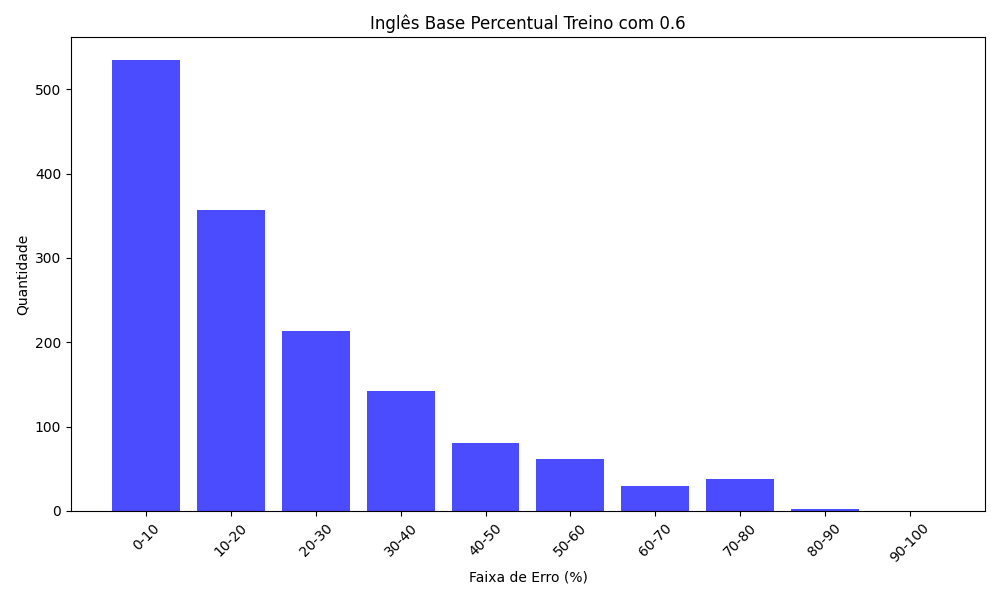
\includegraphics[width=\textwidth]{img/grafsEng/Inglês Base Percentual Treino com 0.6_quantidade.png}
\caption{Quantidade de respostas por faixas de erro percentual dos testes com 40\% do \textit{dataset Mohler} (Inglês) usando o Modelo \textit{BERT Base}}\label{figure:16}
\end{figure}

\begin{figure}[h!]
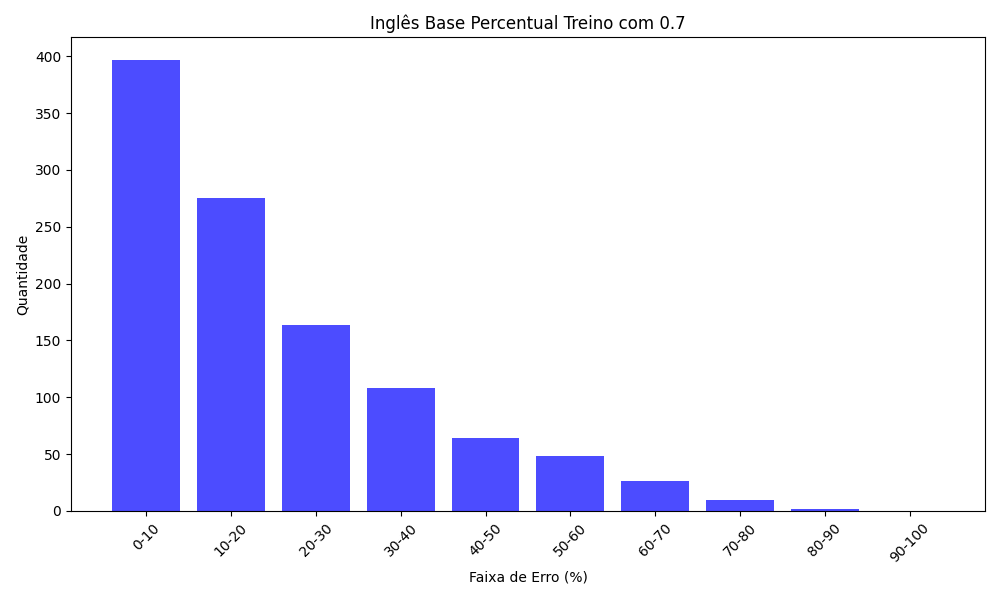
\includegraphics[width=\textwidth]{img/grafsEng/Inglês Base Percentual Treino com 0.7_quantidade.png}
\caption{Quantidade de respostas por faixas de erro percentual dos testes com 30\% do \textit{dataset Mohler} (Inglês) usando o Modelo \textit{BERT Base}}\label{figure:17}
\end{figure}

\begin{figure}[h!]
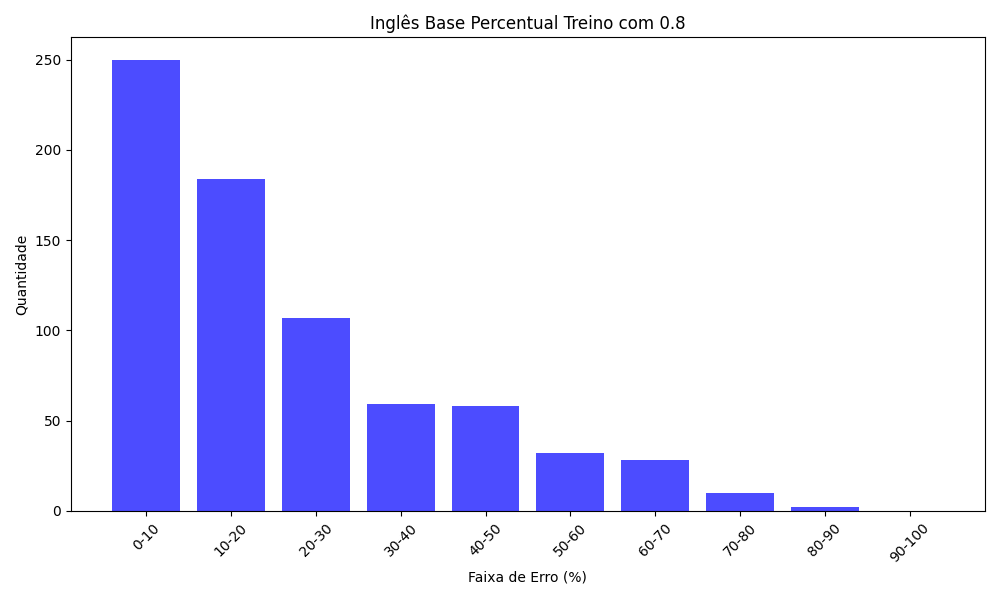
\includegraphics[width=\textwidth]{img/grafsEng/Inglês Base Percentual Treino com 0.8_quantidade.png}
\caption{Quantidade de respostas por faixas de erro percentual dos testes com 20\% do \textit{dataset Mohler} (Inglês) usando o Modelo \textit{BERT Base}}\label{figure:18}
\end{figure}

\begin{figure}[h!]
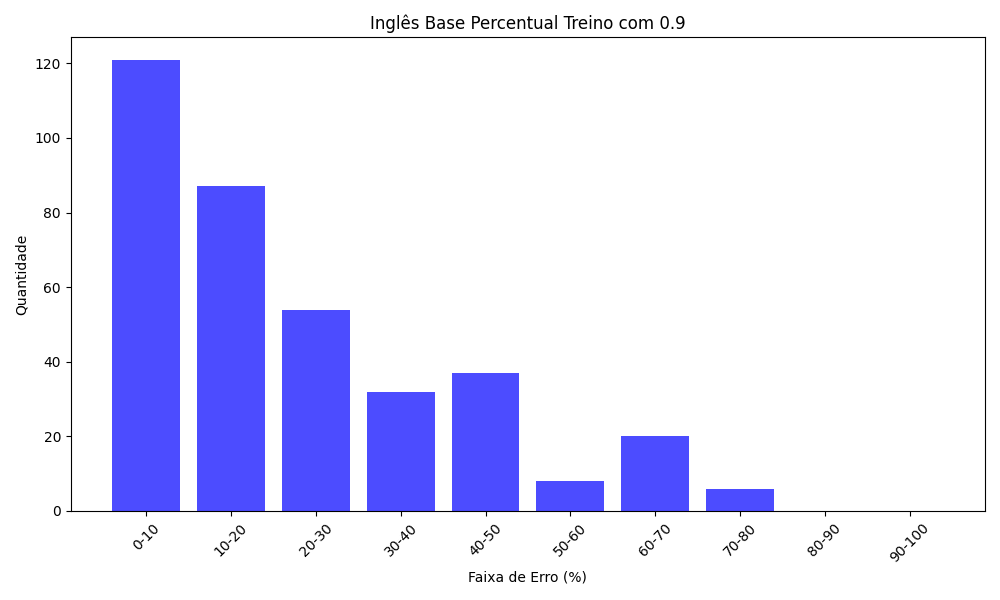
\includegraphics[width=\textwidth]{img/grafsEng/Inglês Base Percentual Treino com 0.9_quantidade.png}
\caption{Quantidade de respostas por faixas de erro percentual dos testes com 10\% do \textit{dataset Mohler} (Inglês) usando o Modelo \textit{BERT Base}}\label{figure:19}
\end{figure}

\FloatBarrier

%--------------------------------------------

\subsection{Resultados do treinamento com o \textit{dataset Mohler} (Inglês) usando o Modelo \textit{BERT Large}}

Os resultados do treinamento com o \textit{dataset Mohler} em inglês utilizando o modelo \textit{BERT Large} indicam uma melhoria geral em comparação ao modelo \textit{BERT Base}. A acurácia média varia de 79.72\% a 81.63\%, mostrando uma maior estabilidade e melhor desempenho com diferentes percentuais de dados de treinamento. Os valores de EQM e EMA também são consistentemente melhores, reforçando a eficácia do modelo \textit{BERT Large}.

\begin{table}[h!]
\centering
\resizebox{\columnwidth}{!}{%
\begin{tabular}{|p{0.25\textwidth}|p{0.1\textwidth}|p{0.1\textwidth}|p{0.4\textwidth}|p{0.1\textwidth}|p{0.1\textwidth}|p{0.1\textwidth}|}
    \hline
    \textbf{Percentual de dados para o treinamento} & \textbf{Qtd. Treino} & \textbf{Qtd. Teste} & \textbf{Pesos [Fator 1, Fator 2, Fator 3]} & \textbf{EQM} & \textbf{EMA} & \textbf{Acurácia} \\
    \hline
     60\% & 2187 & 1459 & [0.4473, 0.1388, 0.1930] & 1.1667 & 0.8519 & 81.19\% \\
    \hline
     70\% & 2552 & 1094 & [0.4698, 0.1487, 0.1814] & 1.1642 & 0.8451 & 81.63\% \\
    \hline
     80\% & 2916 & 730 & [0.4530, 0.1494, 0.1987] & 1.1072 & 0.8240 & 80.68\% \\
    \hline
     90\% & 3281 & 365 & [0.4388, 0.1487, 0.1727] & 1.1034 & 0.8237 & 79.72\% \\
    \hline
\end{tabular}%
}
\caption{Resultados de Regressão para Diferentes Percentuais de Treino com o \textit{dataset Mohler} (Inglês) usando o Modelo \textit{BERT Large}}
\label{tab:resultados_regressao_ingles_large}
\end{table}

Nos gŕaficos das Figuras \ref{figure:20}, \ref{figure:21}, \ref{figure:22} e \ref{figure:23} é possível ver que a maiora das avaliações se mantém na faixa de acurácia acima de 80\%, assim como no modelo \textit{Base}.


\begin{figure}[h!]
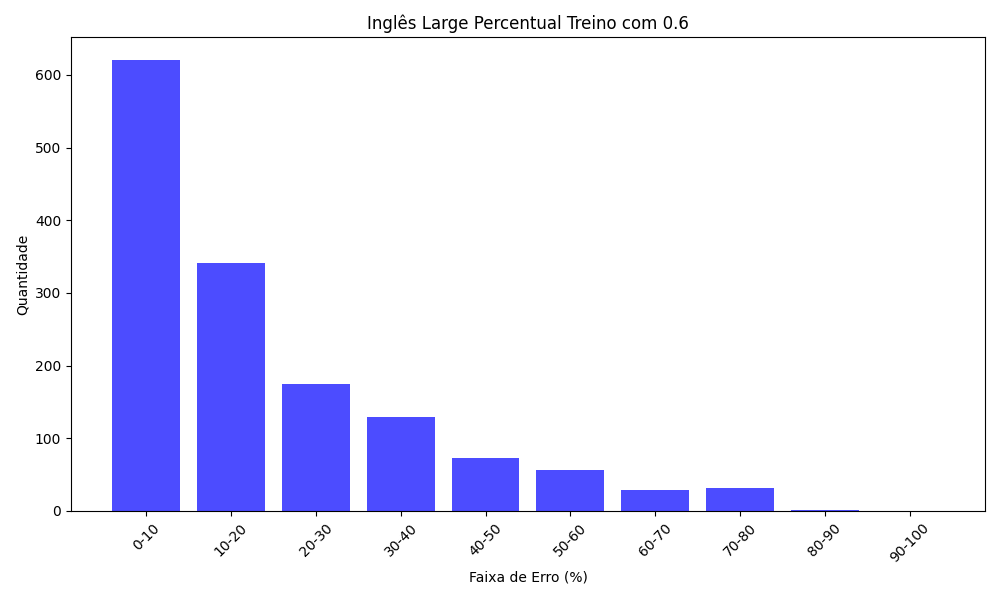
\includegraphics[width=\textwidth]{img/grafsEng/Inglês Large Percentual Treino com 0.6_quantidade.png}
\caption{Quantidade de respostas por faixas de erro percentual dos testes com 40\% do \textit{dataset Mohler} (Inglês) usando o Modelo \textit{BERT Large}}\label{figure:20}
\end{figure}

\begin{figure}[h!]
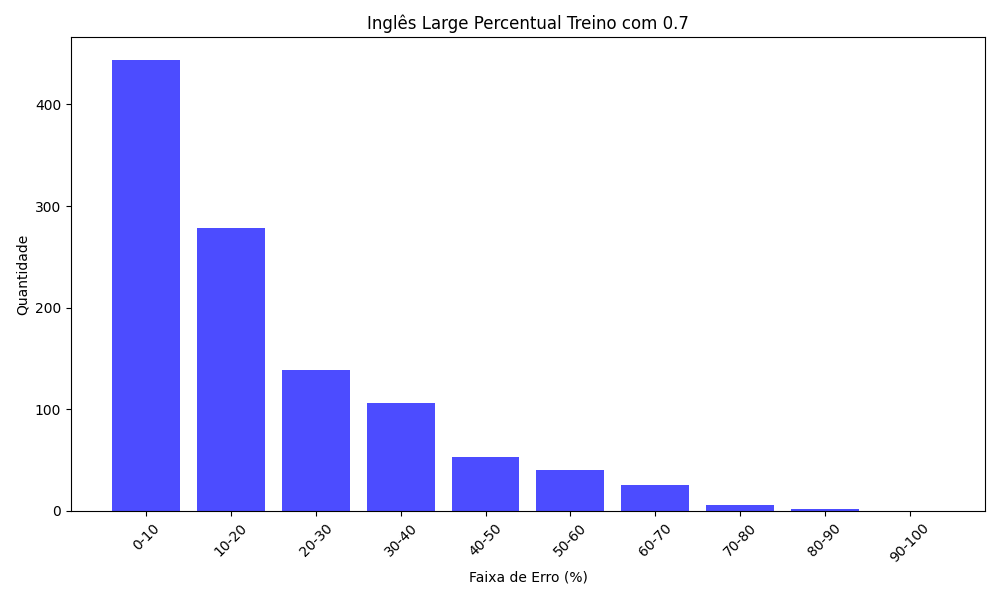
\includegraphics[width=\textwidth]{img/grafsEng/Inglês Large Percentual Treino com 0.7_quantidade.png}
\caption{Quantidade de respostas por faixas de erro percentual dos testes com 30\% do \textit{dataset Mohler} (Inglês) usando o Modelo \textit{BERT Large}}\label{figure:21}
\end{figure}

\begin{figure}[h!]
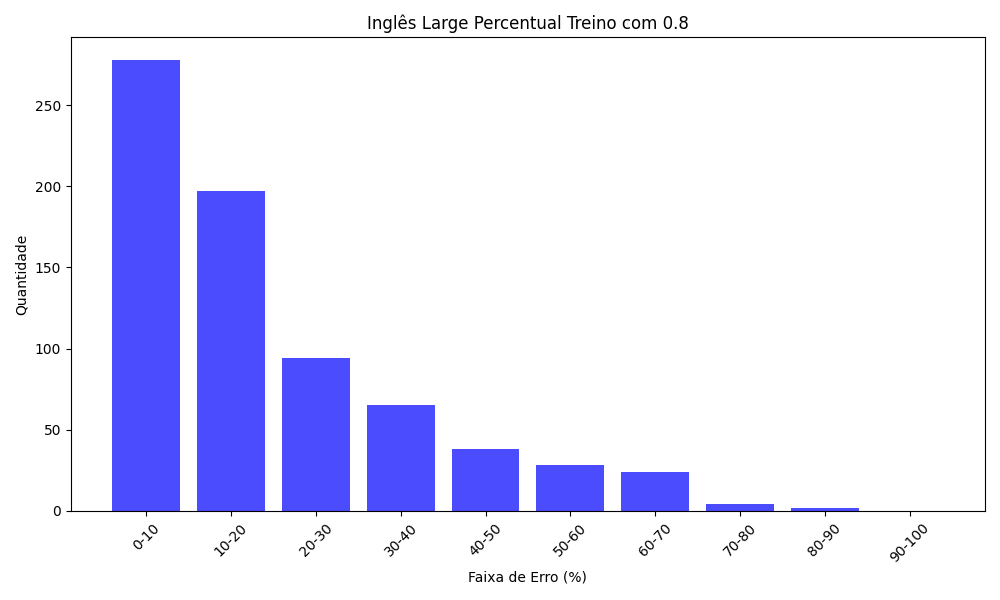
\includegraphics[width=\textwidth]{img/grafsEng/Inglês Large Percentual Treino com 0.8_quantidade.png}
\caption{Quantidade de respostas por faixas de erro percentual dos testes com 20\% do \textit{dataset Mohler} (Inglês) usando o Modelo \textit{BERT Large}}\label{figure:22}
\end{figure}

\begin{figure}[h!]
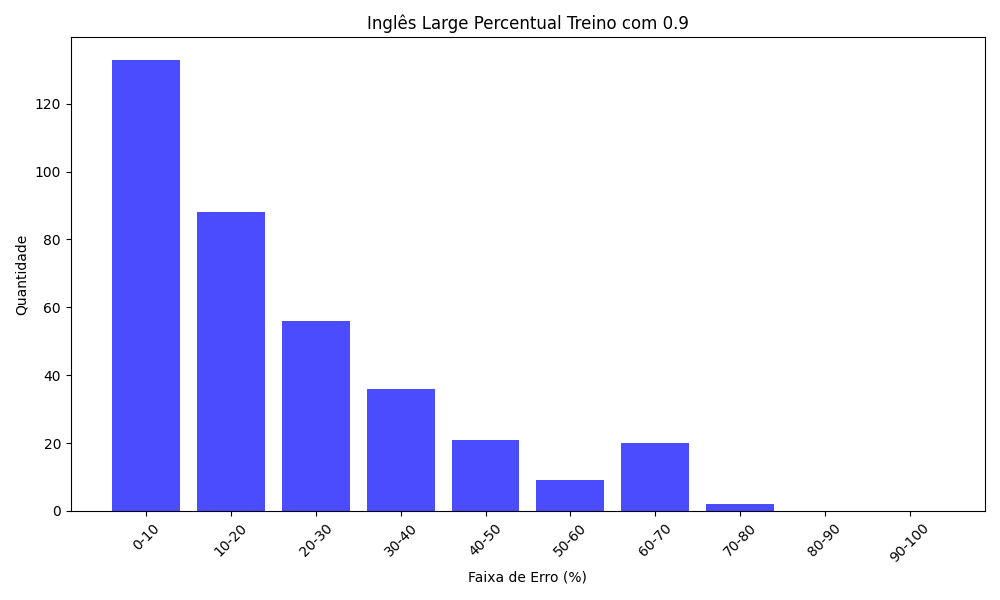
\includegraphics[width=\textwidth]{img/grafsEng/Inglês Large Percentual Treino com 0.9_quantidade.png}
\caption{Quantidade de respostas por faixas de erro percentual dos testes com 10\% do \textit{dataset Mohler} (Inglês) usando o Modelo \textit{BERT Large}}\label{figure:23}
\end{figure}

\FloatBarrier